\chapter{Results: Online Sources}\chlbl{online_sources}
%
\begin{figure}[h]
    \centering
    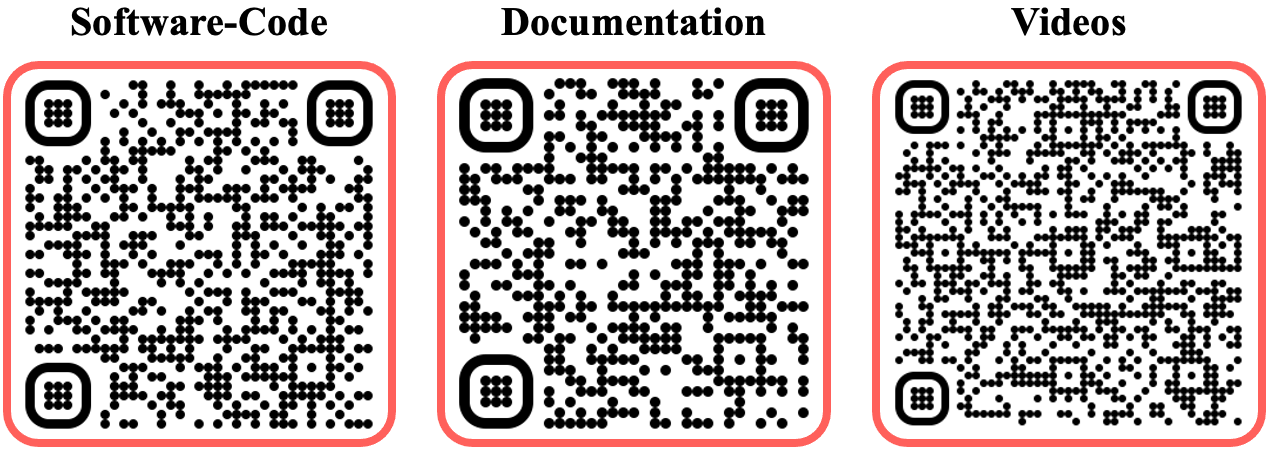
\includegraphics[width=0.79\textwidth]{qr_links}
    \caption[QR-Codes with links to sources]{QR-Codes with links to sources. The first code directs to the Github repository containing the source code, the second code to the repository containing the \LaTeX files to build this documentation, and the third code points to video visualisations of the results.}
    \figlbl{qr_links}
\end{figure}
%
The code and results from this thesis  have been made available as open source on Github: The code is available at \url{https://github.com/sagerpascal/lateral-connections}, and the documentation is available at \url{https://github.com/sagerpascal/msc-thesis}.
Furthermore, a Github webpage provides video visualisations from some of the results at \url{https://sagerpascal.github.io/lateral-connections/results/final_results.html}.
\figref{qr_links} makes these links available as QR codes so that they can easily be accessed with electronic devices.

\section{Video}\chlbl{result_video}
%
\begin{figure}[h]
    \centering
    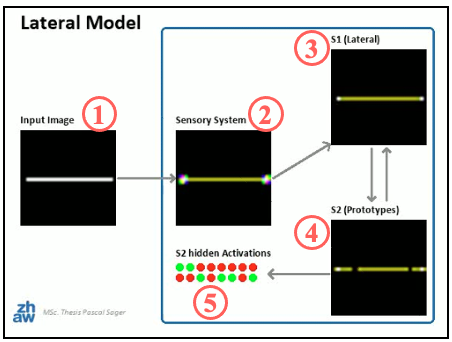
\includegraphics[width=0.99\textwidth]{video_overview}
    \caption[Overview of components visualised in the videos]{An overview of the components visualised in the videos.}
    \figlbl{video_overview}
\end{figure}
%
In the following, the video visualisations accessible at \url{https://sagerpascal.github.io/lateral-connections/results/final_results.html} are explained.
However, the explanations are limited to an overview of which components are shown in each video.
A specific interpretation of the video content is provided in the corresponding result section.

Two video versions are shown for each experiment, both produced by the same model using the same parameter weights.
In the first video version, the Bernoulli neuron is replaced by a neuron using a fixed threshold.
This provides a video output that is more stable and has no flickering activations caused by sampling from a probability distribution.
For the \emph{S0} and \emph{S1} stages, a threshold of $0.5$ is used. Consequently, neurons with a probability of $\geq 0.5$ are set to $1$, while the other neurons are set to $0$.
For the \emph{S2} stage, a threshold of $0.9$ is used, visualising only activities with high certainty that roughly correspond to those accepted by \emph{S1} as feedback signals.
The second video shows the network activities when the Bernoulli neurons are used.

Each video visualises the processing of the input over time.
The first six video frames show how the video is processed over the $T=6$ timesteps of the fast loop, followed by five additional frames depicting the final prediction after the fast loop.
By doing so, viewers have time to analyse the network's activations during this short interruption before the next input is fed into the model and the process repeats.

\figref{video_overview} shows a single video frame, providing an overview of the components displayed in each video:
\begin{enumerate}
    \item The left part of the video displays the input image fed into the sensory system. It is a binary image with one colour channel, whereby active pixels are depicted in white and inactive pixels are depicted in black.
    \item The activations of the sensory system are shown in the middle of the video. The sensory system extracts $4$ features at each location. Each feature combination is visualised in a different colour, and locations without any activations are depicted in black.
    \item \emph{S1} is visualised in the top right corner. It uses the same colours as the sensory system. However, the activations might differ since neurons with insufficient lateral support are turned off.
    \item \emph{S2} is shown in the bottom right corner. It uses the same colours as the sensory system and \emph{L1}. The visualisation depicts the reconstructed version, i.e., the feedback provided to \emph{S1} after mapping \emph{S1}' activities to the latent variables.
    \item The latent variables of \emph{S2} are shown at the center bottom of the video as $16$ circles. Each circle represents a cell, with green indicating an active cell and red indicating an inactive one. 
\end{enumerate}

For a detailed explanation of the content and observations in each video, please refer to the results chapter of this thesis.




